\documentclass[10pt]{article}
\usepackage[margin=1.6cm,top=1.4cm,bottom=1.6cm]{geometry}
\usepackage[T1]{fontenc}
\usepackage{amsmath,amssymb,booktabs,graphicx,xcolor,enumitem,caption,float}
\usepackage[hidelinks]{hyperref}
\setlist{itemsep=1pt,topsep=2pt}
\captionsetup{font=small,labelfont=bf,skip=2pt}
\setlength{\textfloatsep}{6pt}\setlength{\intextsep}{4pt}
\setlength{\parskip}{3pt}
\setlength{\parindent}{0pt}
\setlength{\emergencystretch}{3em}
\definecolor{ink}{HTML}{1B2430}
\definecolor{accent}{HTML}{2A78D6}
\definecolor{good}{HTML}{13865D}
\definecolor{warn}{HTML}{C9551F}
\newcommand{\headline}[2]{\par\medskip{\color{accent}\large\bfseries #1}\par\nopagebreak\vspace{1pt}{\itshape #2}\par\nopagebreak\vspace{2pt}}
\newcommand{\why}[1]{\par\noindent\colorbox{good!8}{\parbox{\dimexpr\textwidth-2\fboxsep}{\small\textbf{Why it matters.} #1}}\par\smallskip}
\newcommand{\solid}[1]{\par\noindent\colorbox{warn!7}{\parbox{\dimexpr\textwidth-2\fboxsep}{\small\textbf{How solid.} #1}}\par\smallskip}
\newcommand{\rtHz}{nV/$\sqrt{\text{Hz}}$}

\begin{document}
\begin{center}
{\LARGE\bfseries What the amplifier traces told us}\\[3pt]
{\large Main results of the amplifier-physics study, in plain terms}\\[3pt]
{\small ccd\_opt\_ml \textperiodcentered{} PA03, boards 101 and 102 \textperiodcentered{} 2026-11-16 (rev.\ 2) \textperiodcentered{} full report: \texttt{docs/overleaf\_amp\_phys\_2026-11-16/amp\_phys.tex}}
\end{center}

\textbf{The idea in one paragraph.} A trace is 0.2\,s of the raw output of one CCD amplifier: every ADC sample of a few
pixels, skip after skip. Normally it is boiled down to one number, the read noise. This study reads physics out of it
instead, helped by \emph{dead channels} (outputs with no working amplifier, which show the electronics alone), the
\emph{level-1 strips} (short acquisitions that record all four amplifiers at once and keep every skip), the board
schematics and the CCD's layout and process recipe. The result: an absolute calibration of the readout, a breakdown of
where the noise comes from, a practical rule for the CDS window, and as-built parameters of each amplifier and CCD,
all from data taken during normal operation.

% ------------------------------------------------------------------------------------------------------------------
\headline{1.\ A free, built-in calibration: a dead channel's resistor noise}{The readout chain was calibrated in absolute
units with no test source.}
A resistor at temperature $T$ produces a voltage noise $\sqrt{4kTR}$ fixed by physics. A dead channel's input sees only
the frontend's load resistor and preamp, 17.1\,\rtHz{} in total. Comparing that known input with the measured ADU gives
the chain's gain: \textbf{0.853\,$\pm$\,0.027 ADU per \textmu V}, against 0.875 from the schematic (2.5\,\% apart). From
it follow the conversion gain, \textbf{1.5--1.6\,\textmu V per electron}, and every noise in physical units.
\begin{figure}[H]\centering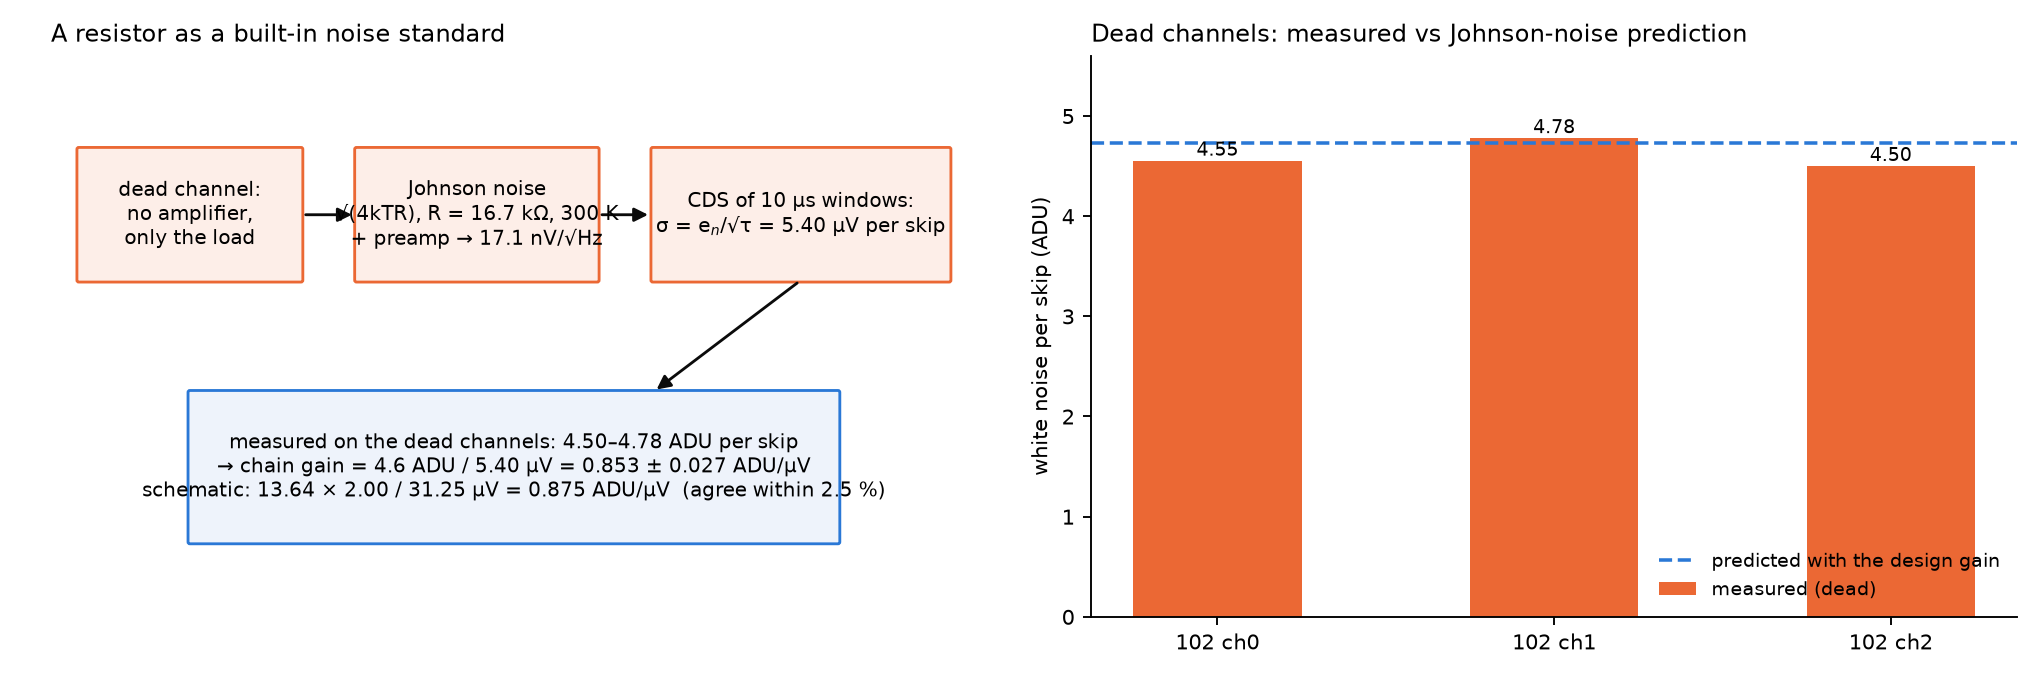
\includegraphics[width=0.5\textwidth]{figures/dead_channel_calibration.png}
\caption{Left: the logic. Right: the three dead board-102 channels (bars) against the Johnson-noise prediction with the
design gain (dashed line).}\end{figure}
\why{Absolute numbers can be compared with the amplifier design and with other systems. One spare unconnected channel per
board makes it a routine check.}
\solid{Solid: two independent routes agree within 2.5\,\%.}

% ------------------------------------------------------------------------------------------------------------------
\headline{2.\ Where the single-skip noise comes from: probably the transistor's 1/f noise}{Not its thermal noise, and not (per
skip) the setup.}
The output transistor's \emph{thermal} noise is at most 4.9\,\rtHz{} at 130\,K; the measured CDS noise is 19--22. The new
handle is the \textbf{CDS window length $\tau$}, which the v2 data varied from 3 to 30\,\textmu s. White noise falls as
$1/\sqrt\tau$ with a longer window; the transistor's 1/f noise (charge hopping in and out of traps in its gate oxide) hardly
changes. Fitting each amplifier's \emph{own} noise (the part not shared with the other three, from the strips) over the
100 v2 strips separates the two:
\begin{itemize}
\item \textbf{Up to 55--80\,\% of the single-skip noise does not shrink with the window} at the present 10\,\textmu s,
  the signature of 1/f noise; the fitted white part is only 9--13\,\rtHz.
\item \textbf{The gate oxides are good:} the implied trap density is at most $\approx2\times10^{16}$\,eV$^{-1}$cm$^{-3}$,
  in the range of good thermal oxide.
\item \textbf{ch2 is the odd one out:} 1.5$\times$ the trap density and twice the 1/f corner (106 vs 34--52\,kHz). This
  ties together its telegraph-like noise, its unstable noise and its doubled noise floor: the amplifier excluded since v1
  has a worse gate oxide. It also shows the only amplifier-linked glow and the largest reset-gate overlap.
\end{itemize}
\why{It explains most of the ``unexplained'' term in the noise budget, and it says what does \emph{not} help: a longer CDS
window (result 3). It also gives a physical reason, not just a statistic, for excluding ch2.}
\solid{The ranking of the amplifiers is robust; the 1/f share and trap density are upper limits. Open: the fitted white
part (9--13) is \emph{below} the 17\,\rtHz{} the frontend alone gives on a dead channel. Either a live transistor shunts the
frontend's noise (which the kTC estimate of result 6 argues against), or the fit counts part of the chain's band-limited
white noise as 1/f. The same fit on the dead channels, plus one DC reading, settle it.}

% ------------------------------------------------------------------------------------------------------------------
\headline{3.\ A practical rule: spend readout time on skips, not on longer windows}{The 10\,\textmu s window is already near
the optimum.}
For a fixed readout time a longer window means fewer skips. Because the 1/f part does not shrink with $\tau$, the noise
reached in a fixed time is lowest at \textbf{5--8\,\textmu s}; the present 10\,\textmu s is within 1--5\,\% of it, and
\textbf{20--30\,\textmu s windows cost 9--32\,\%}. The shared slow noise grows with the window too, so in practice long
windows are worse still.
\begin{figure}[H]\centering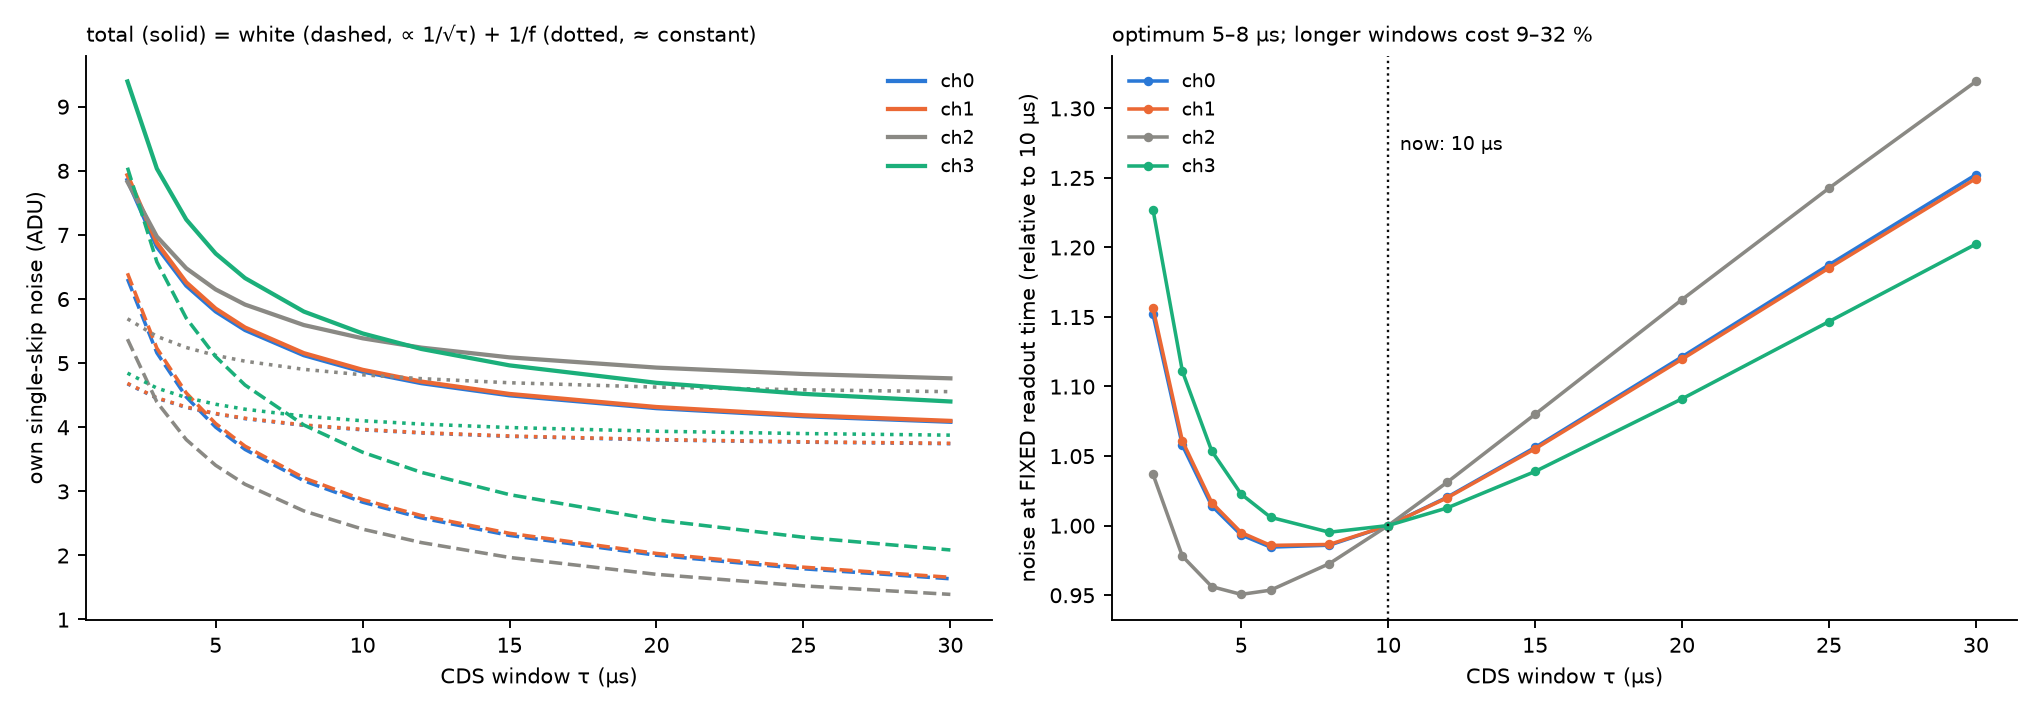
\includegraphics[width=0.74\textwidth]{figures/window_optimum.png}
\caption{Left: each amplifier's own single-skip noise against the window, split into white (dashed) and 1/f (dotted).
Right: the noise reached in a fixed readout time, relative to the present 10\,\textmu s window.}\end{figure}
\why{A direct operating recommendation for v3 and later runs, and it removes long windows from the search space of the
optimisation.}
\solid{Solid: it uses only the measured $\tau$ dependence, not the white/1/f labels. It is computed for each amplifier's own noise; the
500-skip floor is set mostly by shared slow noise, which the cabling (result 4) controls.}

% ------------------------------------------------------------------------------------------------------------------
\headline{4.\ The cabling change, measured three ways}{Shared slow noise fell several-fold; one number now tracks setup quality.}
\textbf{Images} (all four amplifiers read together; empty pixels only; same voltages before and after):
\begin{center}\small
\begin{tabular}{lccc}\toprule
& correlation between amplifiers & read noise ch0 / ch1 & gain from subtracting the common part\\\midrule
October (before) & \textbf{0.19--0.28} & 0.21 / 0.21\,e$^-$ & 5--8\,\%\\
November (after) & \textbf{0.02--0.07} & 0.15 / 0.15\,e$^-$ (\textbf{$-$30\,\%}) & $\approx$0\\\bottomrule
\end{tabular}
\end{center}
\begin{figure}[H]\centering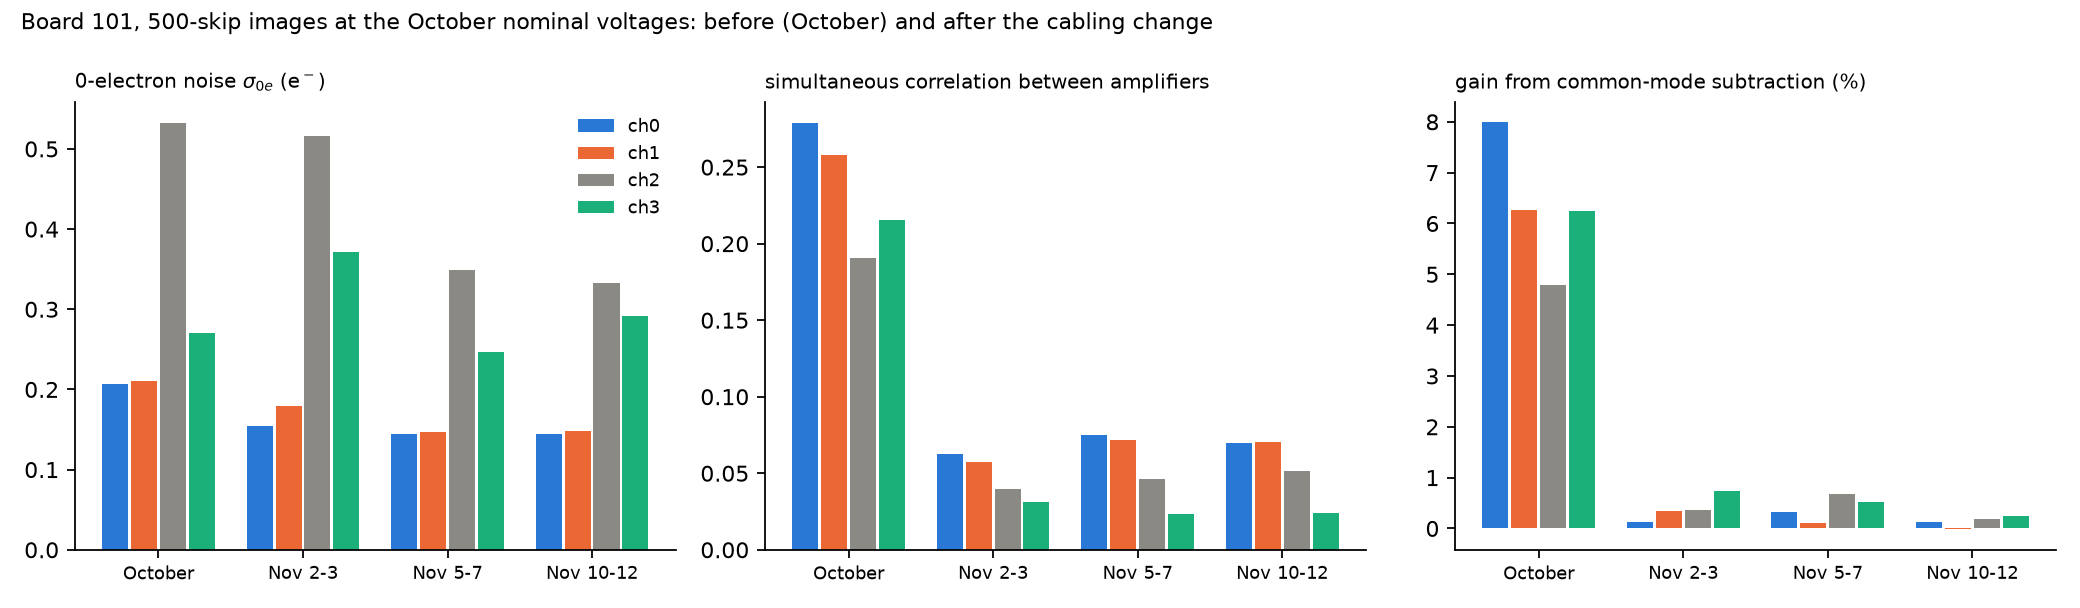
\includegraphics[width=0.64\textwidth]{figures/oct_nov.png}
\caption{Board 101, 500-skip images at the October voltages. Left: the noise of empty pixels per amplifier. Middle: the
correlation between amplifiers. Right: what subtracting the common part would gain.}\end{figure}
\textbf{Level-1 strips} (simultaneous, every skip kept): below 200\,Hz the shared noise power was 23$\times$ each
amplifier's own in October and 3.9$\times$ in November. They also show a \textbf{$\sim$2.5\,kHz interference line} (and its
harmonic) on every channel in both months, source unknown. \textbf{A single trace} against a dead channel shows the same
slow pickup: at 200\,Hz--1\,kHz a live channel is 20--30$\times$ above the electronics, and that excess fell by
$\approx$30\,\% between traces of the same length. The white noise per skip barely moved (2--8\,\%): the change removed
slow \emph{shared} noise, which is what a 500-skip average is sensitive to.
\why{A setup-quality number for any future grounding or cabling test: $\rho_\text{sim}$ from one image (target 0), or the
shared/own ratio below 200\,Hz from one 30\,s strip, with no charge needed.}
\solid{Images: solid for ch0/ch1. Strips: one October acquisition, and its pixels were 6$\times$ longer, so the 23 vs 3.9
is indicative. Single trace: only three October traces match the November length, so this is a supporting check, not the
measurement.}

% ------------------------------------------------------------------------------------------------------------------
\headline{5.\ How strongly every clock line talks to the amplifier, and how much of it is the board}{A per-line coupling map
from the clock edges already in the traces.}
A voltage step on a gate near the sense node pushes a small charge onto it. The CDS cancels these steps, but the raw trace
shows them. Fitting their size against the rail voltages over many settings gives each line's coupling:
\textbf{reset gate 0.15--0.37\,fF}, summing well 0.08--0.13\,fF, horizontal clocks 0.011--0.016\,fF, vertical clocks
$<$0.003\,fF. Subtracting the dead channels separates CCD from board: \textbf{about 70\,\% of the reset-gate ``feedthrough''
is board pickup}, while the horizontal-clock signal is $\sim$90\,\% real coupling through the CCD.
\why{It ranks the supplies by how quiet they must be (VDD noise of only $\sim$0.6\,\textmu V/$\sqrt{\text{Hz}}$ would
add as much as the present read noise; on VSUB it takes $\sim$60) and stops board effects being mistaken for CCD properties.}
\solid{Solid for RG, SW, H and V; the other lines are estimates.}

% ------------------------------------------------------------------------------------------------------------------
\headline{6.\ Inside the chip without cutting it}{Physical device parameters read off routine operating data.}
\begin{itemize}
\item \textbf{Buried-channel depth $\approx$0.6\,\textmu m.} When the reset transistor switches off, about half its channel
  charge lands on the sense node. The jump grows with RG$_\text{high}-$VR at \textbf{2.1--2.4\,fF/V, the same on all four
  CCDs}; the gate reaches buried charge through the oxide and the silicon in series, which gives the depth. The process
  recipe predicts 0.5--0.7\,\textmu m.
\item \textbf{Sense node and follower gain: two routes that disagree.} From the conversion gain and the layout:
  80--90\,fF and gain 0.85. From the reset (kTC) noise frozen on the node each skip, live minus dead: \textbf{$\approx$45\,fF
  and gain 0.44} (preliminary). Which is right matters for result 2.
\item \textbf{A 0.85\,V channel-potential shift on CCD\_B} ($\approx$0.6\,\% of the implant dose), from where the outputs
  change slope as a rail is scanned.
\item \textbf{Between the channels:} crosstalk 1--2$\times10^{-4}$, video-line capacitances 0.1--0.85\,pF and a
  2--4\,$\Omega$ shared return between ch0/ch2 and ch1/ch3, a grounding defect that can be fixed.
\end{itemize}
\why{Depth, dose and node capacitance normally need a sectioned die or a dedicated test structure. Here they come per CCD
from data taken anyway.}
\solid{Model-dependent. The ``half'' charge split is assumed (30--70\,\% gives 0.3--0.9\,\textmu m); oxide thickness and
depth are measured together; the kTC route assumes boards 101 and 102 have the same electronics jitter.}

% ------------------------------------------------------------------------------------------------------------------
\medskip
{\color{accent}\large\bfseries At a glance}\par\vspace{3pt}
\begin{center}\footnotesize\renewcommand{\arraystretch}{1.05}
\begin{tabular}{@{}p{6.3cm}p{6.0cm}p{1.9cm}p{2.6cm}@{}}\toprule
result & value & new? & how solid\\\midrule
chain calibration from a dead channel's resistor noise & 0.853 $\pm$ 0.027 ADU/\textmu V; 1.5--1.6\,\textmu V/e$^-$ & new & solid\\
single-skip noise largely 1/f-like & $\le$55--80\,\%; thermal $\le$4.9 of 19--22\,\rtHz & new & upper limit\\
oxide trap density; ch2 worst & $\lesssim2\times10^{16}$\,eV$^{-1}$cm$^{-3}$; ch2 1.5$\times$ & new & relative indicative\\
optimal CDS window at fixed time & 5--8\,\textmu s; 20--30\,\textmu s costs 9--32\,\% & new & solid (own noise)\\
setup quality before / after the cabling & $\rho_\text{sim}$ 0.25 $\to$ 0.05; $-$30\,\% noise & new metric & solid (ch0/ch1)\\
shared slow noise in strips; interference line & 23$\times$ $\to$ 3.9$\times$ own; 2.5\,kHz & new & indicative\\
clock-line couplings, board vs CCD & RG 0.15--0.37\,fF; 70\,\% of RG is pickup & new & solid\\
buried-channel depth & $\approx$0.6\,\textmu m (0.3--0.9) & new & model\\
sense node, follower gain & 80--90\,fF / 0.85 vs 45\,fF / 0.44 & new routes & open\\
crosstalk, line capacitance, shared return & $10^{-4}$; 0.1--0.85\,pF; 2--4\,$\Omega$ & partly new & indicative\\\bottomrule
\end{tabular}
\end{center}

{\color{accent}\large\bfseries What would firm it up}\par\vspace{2pt}
\begin{enumerate}
\item \textbf{The DC level of each video line} (or the VDD current). It now decides three things at once: the sense-node
  capacitance (45 or 85\,fF), the white/1/f split of result 2, and the absolute trap density.
\item \textbf{The window fit on the dead channels} (existing v2 strips): no transistor, so it should find no 1/f.
\item \textbf{Find the 2.5\,kHz line} (a switching converter or a periodic digital process), with one strip per suspect.
\item \textbf{Telegraph steps in ch2's raw traces}: their size against one trapped charge would locate the trap directly.
\item \textbf{A second module}: checks that the methods carry over and how much CCDs differ.
\end{enumerate}

\end{document}
